\documentclass{article}

\usepackage{listings}
\usepackage{xcolor}
\usepackage{geometry}

\usepackage{graphicx}
\usepackage{subcaption}
\usepackage{float}
\usepackage{booktabs}
\usepackage{hyperref}


\geometry{a4paper, margin=1in}

\lstset{
  basicstyle=\small\ttfamily,
  keywordstyle=\color{blue},
  commentstyle=\color{green!40!black},
  stringstyle=\color{orange},
  numbers=left,
  numberstyle=\tiny\color{gray},
  breaklines=true,
  frame=single,
  tabsize=2,
  captionpos=b
}

\title{Report - CG: Bonus Assignment 2}
\author{Jeferson Morales Mariciano, Martin Lettry}
\date{\today}

\begin{document}

\maketitle

\section*{Prerequisites:}
Before running the code, please download the meshes from the iCorsi link:\\
\url{https://www.icorsi.ch/pluginfile.php/1610541/mod_assign/introattachment/0/spatial_data_structures.zip?forcedownload=1}\\
and put it inside the \textit{./code} folder and keep it with the name \textit{meshes/} to have the paths
like \textit{./meshes/armadillo.obj} for \textit{main.cpp} to run properly.\\
Such files were not included because to large for iCorsi submissions.\\

The \textit{run.sh} contains the script use for the benchmarking, which correspond to the script written in the assignment
for evaluation.\\
For benchmarking:
\begin{itemize}
  \item the mesh load time is not counted, only the image rendering time is
  \item the resolution is set to $2048 \times 1536$
  \item the assignment command for benchmarking was used inside \textit{run.sh}
  \item single thread implementation
\end{itemize}


\section*{Summary of Implementation:}
We implemented two structures:
\begin{itemize}
  \item \texttt{AABB} (Axis-Aligned Bounding Box) for completing \underline{Version A} of the assignment.
  \item \texttt{BVHNode} (Bounding Volume Hierarchy Node) for completing \underline{Version B} of the assignment.
\end{itemize}

For all benchmarks, including the final \textit{result.ppm} both techniques have been implemented:
in last notes on Table \ref{tab:scene-timing} show the total time to render the scene using both techniques
with and without shading effects, specifically this effect due to time complexity spike.\\


\begin{lstlisting}[language=C++]
struct AABB
{
  glm::vec3 min;
  glm::vec3 max;
};

struct BVHNode
{
  AABB bounds;
  vector<Triangle> triangles;
  BVHNode *left;
  BVHNode *right;
};
\end{lstlisting}

When loading a \texttt{Mesh} object, the BVH implementation is optional.

If chosen, the BVH is constructed by recursively splitting triangles along the center of mass,
alternating among $x, y, z$ axes.
The process continues until each \texttt{BVHNode} contains a maximum of $n$ triangles, which for our implementation
is chosen to be $n=20$.\\

Logic steps:
\begin{itemize}
  \item When computing the ray-mesh intersection, the algorithm checks whether the BVH implementation is active.
  \item If not, it checks if the ray is within the mesh bounding box and computes intersections with individual triangles as in assingnment bonus 1.
  \item With BVH, the algorithm recursively checks intersections with bounding boxes, descending until leaf nodes are reached using the BVH data structure.
  \item Finally, it computes intersections with triangles and returns the closest one.
\end{itemize}

We also created a small python file \textit{report.py} to help with plotting the data.
It generated the below plot, which shows the render time as a function of the number of triangles in the mesh.

\section*{Implementation Issues:}

One issue we faced was regarding the special corner case of intersection between the ray
and both the right and left child nodes.\\
This can happen if the triangle overlaps the splitting plane, in which case we need to recursively
traverse both the left and right node to find the correct intesected one.\\

Another issue we faced is due to time complexity of shadowing.\\
We have both stats of the rendered image with and without shadowing and we see that without such effect
we get similar stats of what the assignment asked for: around $\approx 15$ seconds.\\
However, when we add shadowing, the time complexity increases a lot, and we get around $\approx 50$ seconds.\\


\section*{Benchmarking results:}

Nevertheless, both Table \ref{tab:no-shadow}, \ref{tab:shadow} show from raw data a sublinear relationship
between the number of triangles and the render time if taking in consideration the same mesh rendered.\\


\begin{table}[h]
  \centering
  \caption{Performance Data - no shadowing}
  \label{tab:no-shadow}
  \begin{tabular}{lcc}
    \toprule
    \textbf{Mesh}    & \textbf{Size (in Triangles)} & \textbf{Time to render (s)} \\
    \midrule
    armadillo\_small & 3112                         & 2.45998                     \\
    lucy\_small      & 2804                         & 2.92673                     \\
    bunny\_small     & 1392                         & 1.73724                     \\
    armadillo        & 345944                       & 3.96717                     \\
    lucy             & 2805572                      & 14.3597                     \\
    bunny            & 69451                        & 1.95838                     \\
    \bottomrule
  \end{tabular}
\end{table}


\begin{figure}[H]
  \caption{Render Time by Number of Triangles - no shadowing}
  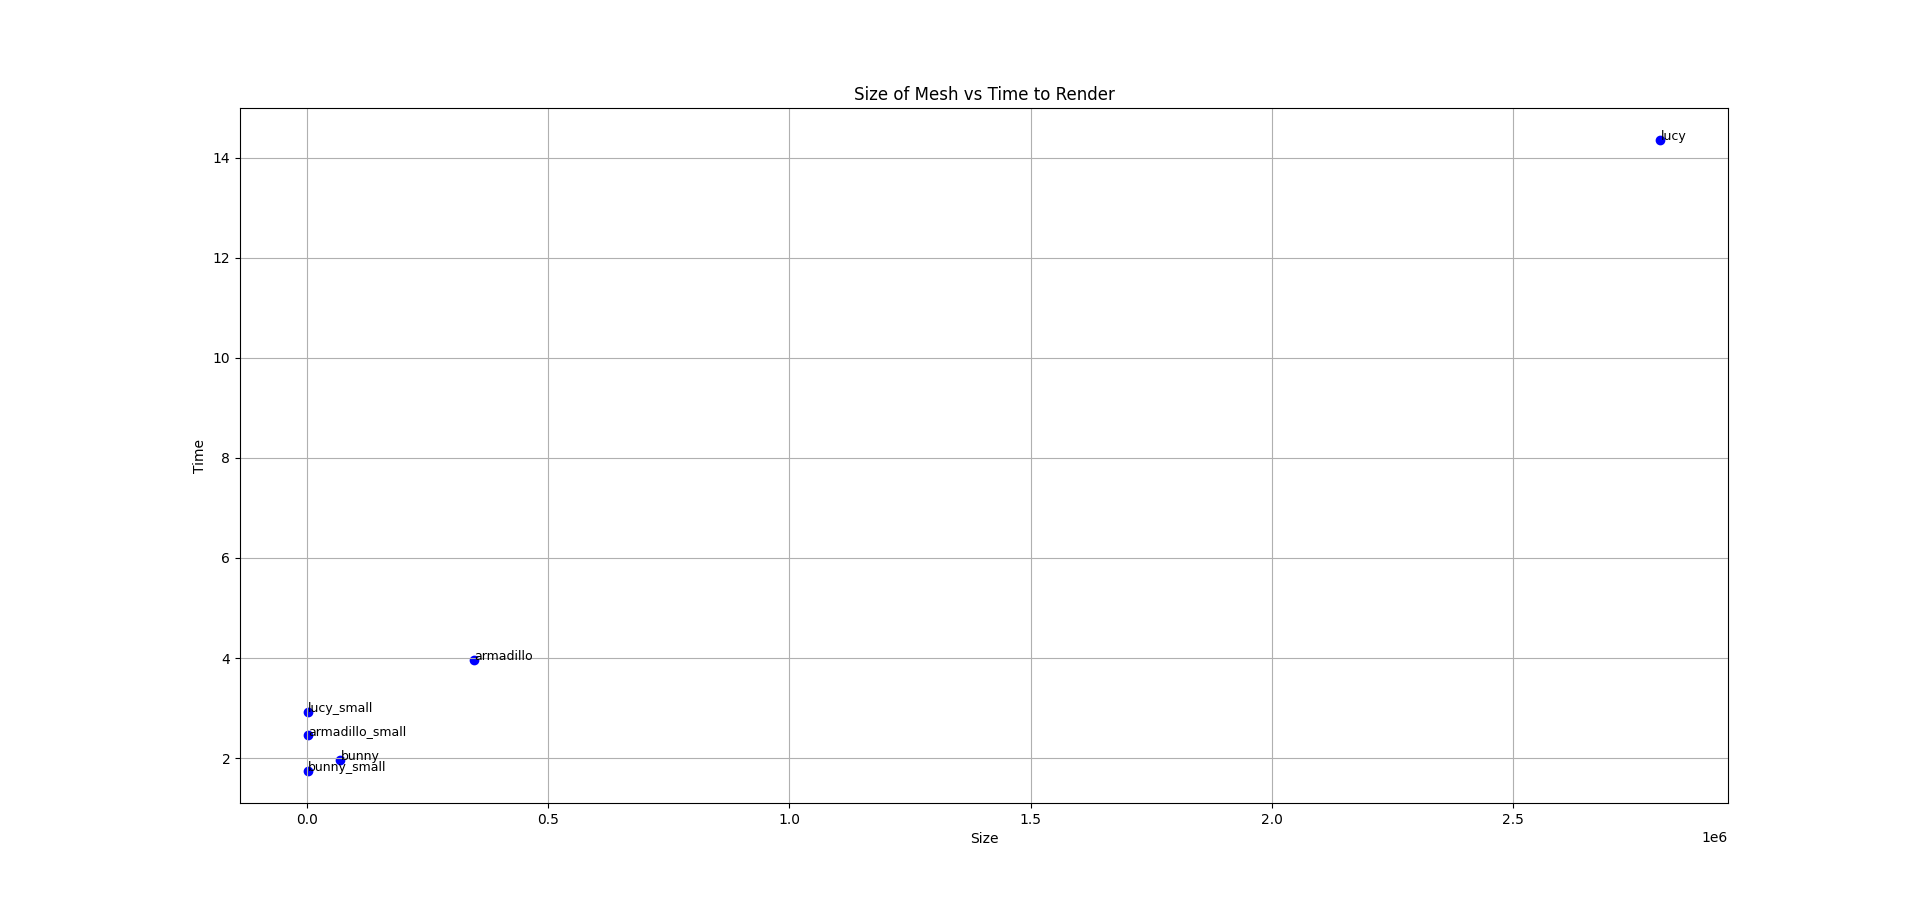
\includegraphics[width=\linewidth, trim={5cm 0cm 4cm 0cm}, clip]{Figure_1.png}
\end{figure}


As expected, we can observe a sub-linear relationship between the number of triangles and the render time.\\
meaning that the slop connecting the same pair of mesh small-large is visibly smaller than 1.\\

\begin{table}[h]
  \centering
  \caption{Performance Data - with shadowing}
  \label{tab:shadow}
  \begin{tabular}{lcc}
    \toprule
    \textbf{Mesh}    & \textbf{Size (in Triangles)} & \textbf{Time to render (s)} \\
    \midrule
    armadillo\_small & 3112                         & 12.2288                     \\
    lucy\_small      & 2804                         & 13.9946                     \\
    bunny\_small     & 1392                         & 5.54895                     \\
    armadillo        & 345944                       & 17.043                      \\
    lucy             & 2805572                      & 33.7117                     \\
    bunny            & 69451                        & 8.2359                      \\
    \bottomrule
  \end{tabular}
\end{table}


\begin{figure}[H]
  \caption{Render Time by Number of Triangles - with shadowing}
  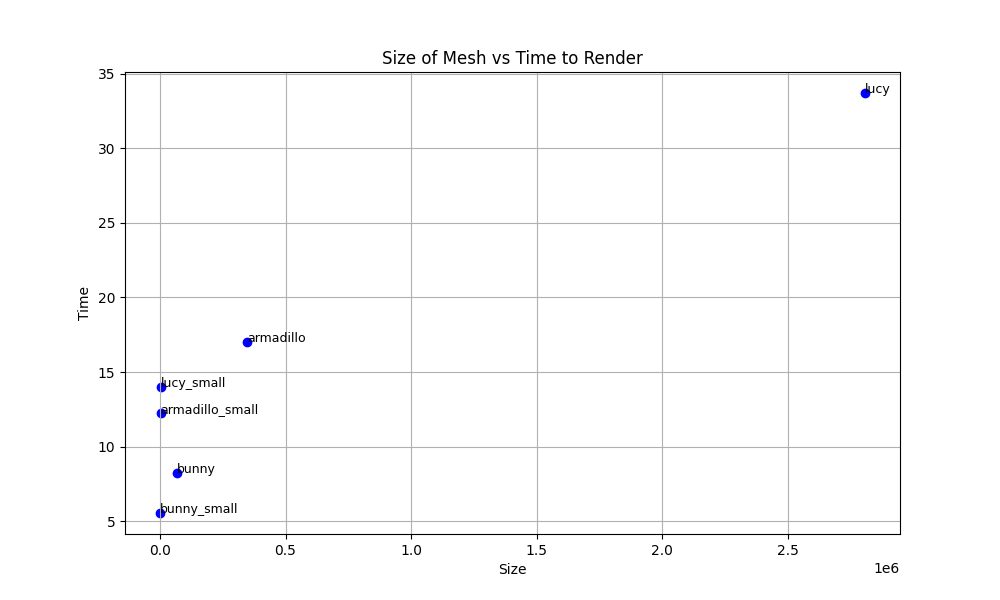
\includegraphics[width=\linewidth, trim={3cm 0cm 3cm 0cm, clip}]{Figure_2.png}
\end{figure}

The total time to render the assignment scene with large meshes of \textit{armadillo}, \textit{lucy} and \textit{bunny}
in $2048 \times 1536$ resolution:

\begin{table}[H]
  \caption{Scene timing benchmarks}
  \label{tab:scene-timing}
  \centering
  \begin{tabular}{|l|l|} \hline\hline
    no shadowing         & shadowing            \\ \hline
    $\approx 14$ seconds & $\approx 50$ seconds \\ \hline \hline
  \end{tabular}
  \label{table:rec_p16}
\end{table}

You can change it and verify it easily in the scene definition function in \textit{main.cpp}.

\section*{Further possible improvement analyzation}

Implementing Sphere box or even better convex hulls instead of bounding box could greatly improve performance.\\
Also, implementing a more advanced version of BVH spatial data structure could dramatically improve performance.\\

\end{document}
